\documentclass[aspectratio=169,table]{beamer}

\usepackage{graphicx}
\usepackage{import}
\usepackage{media9}
\usepackage{multimedia}
\usepackage{pifont}% http://ctan.org/pkg/pifont
\newcommand{\cmark}{\ding{51}}%
\newcommand{\xmark}{\ding{55}}%
\newcommand{\gcmark}{{\color{green}\cmark}}%
\newcommand{\ycmark}{{\color{yellow}\cmark}}%
\newcommand{\rxmark}{{\color{red}\xmark}}%
\usepackage{tikz}

\usetikzlibrary{3d}
\usetikzlibrary{backgrounds}
\usetikzlibrary{decorations.pathreplacing}
\usetikzlibrary{fit}
% \usetikzlibrary{external}
\usetikzlibrary{matrix}
\usetikzlibrary{positioning}
\usetikzlibrary{scopes} % brilliant library!
\usetikzlibrary{tikzmark}

% \tikzexternalize

\pgfdeclarelayer{background}
\pgfdeclarelayer{foreground}
\pgfsetlayers{background,main,foreground}


\usetheme{Janelia}

\setbeamercolor{description item}{fg=HHMIGreenB}

\title[Janelia Theme]{The Metamorphosis of BigCAT --- Proofreading Experiments\\}
\subtitle{Proofreading Experiments}
% \subtitle{A custom modern minimalist Beamer theme designed from scratch}
\author{Philipp Hanslovsky}
\date{February 8, 2018}

\setcounter{showSlideNumbers}{1}

\begin{document}

\setcounter{showProgressBar}{0}
\setcounter{showSlideNumbers}{0}

\frame{\titlepage}

\begin{frame}
    \frametitle{Circuit Reconstruction}
    \begin{tikzpicture}
        \node[] (diagram) {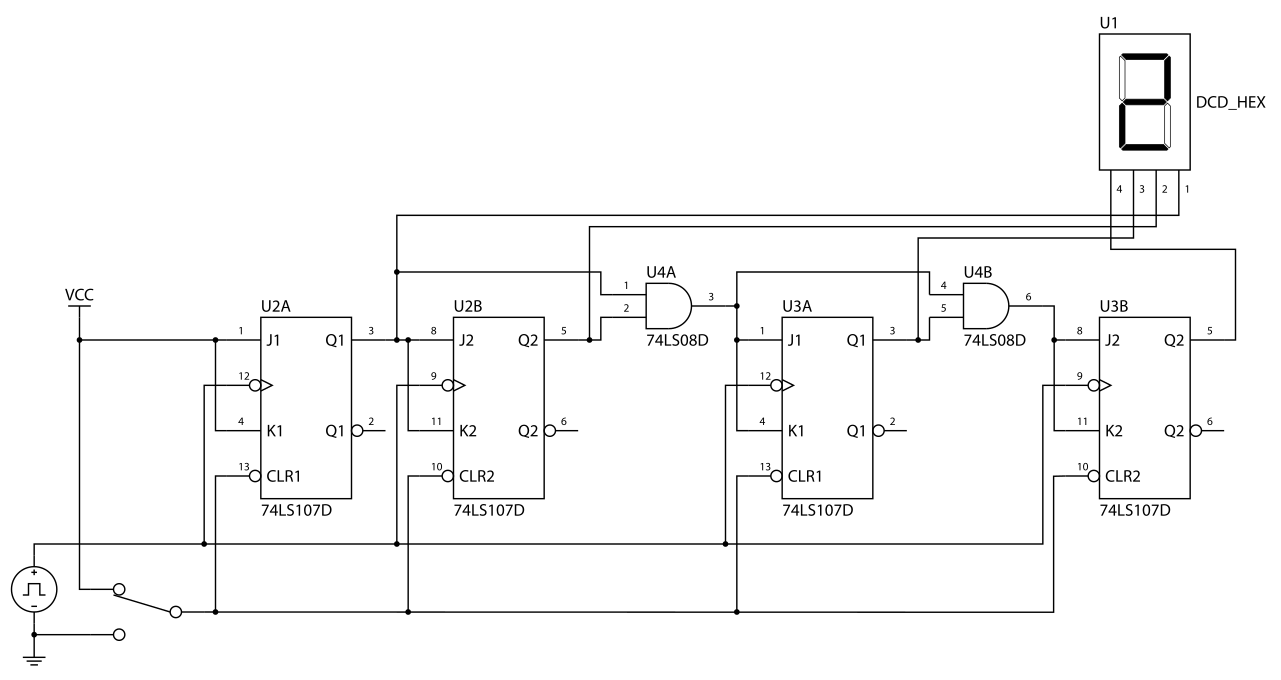
\includegraphics[width=0.4\textwidth]{fig/circuit-diagram.pdf}};
        \node[anchor=north,font=\tiny] at (diagram.south) {https://upload.wikimedia.org/wikipedia/commons/7/76/4\_bit\_counter.svg};%% https://upload.wikimedia.org/wikipedia/commons/7/76/4_bit_counter.svg};
        % \begin{scope}[x={(diagram.south east)},y={(diagram.north west)}]
        %     \visible<2->{
        %     \draw[red] (0.5,0.2) ellipse (2mm and 5mm);
        % }
        % \end{scope}
    \visible<2->{
            \node[anchor=west,inner sep=0] (neuron) at ([xshift=30]diagram.north east) {\includegraphics[width=0.3\linewidth]{fig/neuron.png}};
            \node[anchor=north,font=\tiny] at (neuron.south) {https://www.wikipedia.org/};
        }
        \visible<3-> {
            % https://upload.wikimedia.org/wikipedia/commons/thumb/b/bc/Neuron_Hand-tuned.svg/400px-Neuron_Hand-tuned.svg.png
            \node[anchor=west] (synapse) at ([xshift=60]diagram.south east) {\includegraphics[width=0.1\linewidth]{fig/synapse.png}};
            \node[anchor=north,font=\tiny] at (synapse.south) {https://psychlopedia.wikispaces.com};
            % https://psychlopedia.wikispaces.com/file/view/syn.gif/325862020/syn.gif
        }
        \end{tikzpicture}
\end{frame}

\begin{frame}
    \frametitle{Automatic Reconstruction}

    \begin{textblock}{3}(11.4,0)
        \tiny\includegraphics[width=1cm]{fig/people/funke.png}
        
        J. Funke%
    \end{textblock}%
    
    \begin{textblock}{3}(12.6,0)
        \tiny\includegraphics[width=1cm]{fig/people/papec.png}

        C. Pape%
    \end{textblock}%
    
    \begin{textblock}{3}(13.8,0)
        \tiny\includegraphics[width=1cm]{fig/people/tschopp.jpeg}

        F. Tschopp%
    \end{textblock}%
    
    \begin{textblock}{3}(15,0)
        \tiny\includegraphics[width=1cm]{fig/people/turaga.jpg}

        S. Turaga%
    \end{textblock}%

    \vspace{1cm}
    \begin{tikzpicture}[remember picture]
        \node[anchor=south west] (pipeline) {\includegraphics{fig/reconstruction-pipeline.pdf}};
        \begin{scope}[x={(pipeline.south east)},y={(pipeline.north west)}]
            \coordinate (boundary) at (0.22, 0.2);
            \coordinate (agglomeration) at (0.77, 0.2);
            \visible<2->{
                \node[red,ultra thick] (ml) at (0.5,-0.2) {Machine Learning};
                \draw[red,ultra thick] (0.22,0.5) ellipse (0.07 and 0.25);
                \draw[thick,red] (ml.west) edge [->,out=180,in=270] (boundary);

                
                
                
            }
            \visible<3->{
                \draw[red,ultra thick] (0.77,0.5) ellipse (0.07 and 0.25);
                \draw[thick,red] (ml.east) edge [->,out=0,in=270] (agglomeration);
            }
        \end{scope}
    \end{tikzpicture}

    
    \begin{tikzpicture}[remember picture,overlay]
        \visible<2-> {
            \draw[thick,red]  ([xshift=-15,yshift=5]pic cs:funke) edge[->,in=250,out=150] ([xshift=-5]boundary);
        }
        \visible<3-> {
            \coordinate (inBetween) at ([xshift=70,yshift=3]$(pic cs:beier)!0.5!(pic cs:pape)$);
            \draw[thick,red] ([yshift=3]pic cs:beier) edge[in=210,out=0] (inBetween);
            \draw[thick,red] ([yshift=3]pic cs:pape) edge[in=210,out=0] (inBetween);
            \draw[thick,red] (inBetween) edge[->,in=290,out=30] ([xshift=5]agglomeration);
            % \draw[thick,red]  ([xshift=-15,yshift=5]pic cs:funke) edge[->,in=250,out=150] ([xshift=-5]boundary);
        }
    \end{tikzpicture}

    \vspace{1cm}
    \visible<1->{
        \tiny 
        \begin{enumerate}[(1)]
              \item \tikzmark{funke} Funke \emph{et al.} ``A deep structured learning approach toward automating connectome reconstruction from 3D electron micrographs'' (2017). arXiv 1709.0297
              \item Beier \emph{et al.} ``Multicut brings automated neurite segmentation closer to human performance'' (2017). Nature methods 4, 101-102 \tikzmark{beier}
              \item Pape \emph{et al.} ``Solving large Multicut problems for connectomics via domain decomposition'' (2017) ICCV. \tikzmark{pape}
        \end{enumerate}
        % \begin{tikzpicture}[remember picture]\coordinate (funke) at (0,0);\end{tikzpicture}
        
    }

\end{frame}


\begin{frame}
    \frametitle{CREMI}
    \only<1>{
        \begin{tikzpicture}[remember picture,overlay]
            \node[] at (current page.center) {\includegraphics[width=\paperwidth]{fig/cremi.png}};
        \end{tikzpicture}
    }

    \only<2>{
        \vspace{1cm}
        \includegraphics[width=\columnwidth]{fig/challenge-pixels-2.pdf}
    }

    \begin{textblock}{3}(11.4,0)
        \tiny\includegraphics[width=1cm]{fig/people/funke.png}
        
        J. Funke%
    \end{textblock}%
    
    \begin{textblock}{3}(12.6,0)
        \tiny\includegraphics[width=1cm]{fig/people/bock.jpeg}
        
        D. Bock%
    \end{textblock}%
    
    \begin{textblock}{3}(13.8,0)
        \tiny\includegraphics[width=1cm]{fig/people/perlman.jpeg}
        
        E. Perlman%
    \end{textblock}%
    
    \begin{textblock}{3}(15,0)
        \tiny\includegraphics[width=1cm]{fig/people/turaga.jpg}
        
        S. Turaga%
    \end{textblock}%
    
    \begin{textblock}{3}(0.5,14)
        {\color{white}\Huge\bf cremi.org}
    \end{textblock}
\end{frame}


\begin{frame}
    \frametitle{BigCAT}
    % \begin{itemize}
    %       \item Arbitrary Re-Slicing
    %       \item Painting (!!)
    %       \item Agglomeration
    %       \item Annotations
    %       \item Potential for heavy workload tasks on client
    % \end{itemize}

    \begin{tikzpicture}[remember picture,overlay]
        \node[fit=(current page),fill=black,inner sep=0] {};
    \end{tikzpicture}%
    \def\factor{1.0}

    \visible<1-2>{
    \movie[%
    % width=\factor\textwidth,%
    % height=\factor\textheight,%
    ]{\includegraphics[width=\factor\textwidth]{vid/bigcat-cremi-placeholder.jpg}}{vid/bigcat-cremi-b-aligned.mov}
    }

    

    \only<1>{
        % \includegraphics[width=\factor\textwidth]{vid/bigcat-cremi-placeholder.jpg}
        \begin{textblock}{3}(13.8,0)
            \tiny\includegraphics[width=1cm]{fig/people/funke.png}
        
            {\color{white}J. Funke}%
        \end{textblock}%
    
        \begin{textblock}{3}(15,0)
            \tiny\includegraphics[width=1cm]{fig/people/pietzsch.png}
        
            {\color{white}T. Pietzsch}%
        \end{textblock}%
    }
    
\end{frame}

\begin{frame}
    \frametitle{Required Features}
    \small
    \vspace{1cm}
    \begin{table}
        \centering
        \begin{tabular}{lccc}
          \visible<1->{                             & BigCAT & Neuroglancer\footnote{\tiny{}https://github.com/google/neuroglancer} & BigCAT v2 \\}                       
          \visible<2->{Arbitrary cross-sections     & \gcmark & \gcmark & \gcmark \\}                             
          \visible<3->{Orthogonal views             & \rxmark & \gcmark & \gcmark \\}                             
          \visible<4->{3D visualization             & \rxmark & \gcmark & \gcmark \\}                             
          \visible<5->{3D model generation          & \rxmark & \rxmark & \gcmark \\}                             
          \visible<6->{Painting                     & \gcmark & \rxmark & \gcmark \\}                             
          \visible<7->{Multi-resolution painting         & \rxmark & \rxmark & \gcmark \\}                             
          \visible<8->{Semi-automatic agglomeration & \rxmark & \rxmark & \gcmark \\}                             
          \visible<9->{Extensibility                & \rxmark & \only<9>{\gcmark}\only<10->{\ycmark} & \gcmark \\}
        \end{tabular}
    \end{table}%
    \visible<10>{%
        \begin{tikzpicture}[overlay]%
            \begin{scope}[overlay]
                \node[draw=black] at (10cm,0cm) {\includegraphics[width=3cm]{fig/chrome-heap-limit.png}};%
            \end{scope}
        \end{tikzpicture}%
    }%
\end{frame}

\begin{frame}
    \frametitle{Agglomeration}
    \small
    \vspace{1cm}
    \begin{table}
        \centering
        \begin{tabular}{lccc}
                                       & BigCAT & Neuroglancer & BigCAT v2 \\
          Arbitrary cross-sections     & \gcmark & \gcmark & \gcmark \\
          Orthogonal views             & \rxmark & \gcmark & \gcmark \\ 
          3D visualization             & \rxmark & \gcmark & \gcmark \\ 
          3D model generation          & \rxmark & \rxmark & \gcmark \\ 
          Painting                     & \gcmark & \rxmark & \gcmark \\ 
          Multi-resolution painting         & \rxmark & \rxmark & \gcmark \\ 
          \rowcolor{black!20} Semi-automatic agglomeration & \rxmark & \rxmark & \gcmark \\ 
          Extensibility                & \rxmark & \ycmark & \gcmark \\
        \end{tabular}
    \end{table}
\end{frame}

\begin{frame}
    \frametitle{Agglomeration}
    \begin{tikzpicture}[remember picture,overlay]
        \node[fit=(current page),fill=black,inner sep=0] {};
    \end{tikzpicture}%
    
    \def\factor{0.9}

    % force two slides
    \visible<1-2>{}
    \movie[%
    % width=\factor\textwidth,%
    % height=\factor\textheight,%
    % ]{}{vid/assignments.mp4}
    ]{\includegraphics[width=\factor\textwidth]{vid/assignments-placeholder.jpg}}{vid/assignments.mp4}
    % show video
    % backend: c9ae08b
    % bigcat:  e84388e
    % start with fragment 2660 (blue)

    \only<1>{
    \begin{textblock}{3}(15,0)
        \tiny\includegraphics[width=1cm]{fig/people/papec.png}

        {\color{white}C. Pape}%
    \end{textblock}%
    }
\end{frame}

\begin{frame}
    \frametitle{Multi-Resolution Painting}
    \small
    \vspace{1cm}
    \begin{table}
        \centering
        \begin{tabular}{lccc}
                                       & BigCAT & Neuroglancer & BigCAT v2 \\
          Arbitrary cross-sections     & \gcmark & \gcmark & \gcmark \\
          Orthogonal views             & \rxmark & \gcmark & \gcmark \\ 
          3D visualization             & \rxmark & \gcmark & \gcmark \\ 
          3D model generation          & \rxmark & \rxmark & \gcmark \\ 
          \rowcolor{black!20} Painting                     & \gcmark & \rxmark & \gcmark \\ 
          \rowcolor{black!20} Multi-resolution painting         & \rxmark & \rxmark & \gcmark \\ 
          Semi-automatic agglomeration & \rxmark & \rxmark & \gcmark \\ 
          Extensibility                & \rxmark & \ycmark & \gcmark \\
        \end{tabular}
    \end{table}
\end{frame}

\begin{frame}
    \frametitle{Multi-Resolution Painting}
    
    \begin{tikzpicture}[remember picture,overlay]
        \node[fit=(current page),fill=black,inner sep=0] {};
    \end{tikzpicture}%

    \centering

    \def\factor{0.9}
    \movie[%
    % width=\factor\textwidth,%
    % height=\factor\textheight,%
    % ]{}{vid/paint.mp4}
    ]{\includegraphics[width=\factor\textwidth]{vid/paint-placeholder.jpg}}{vid/paint.mp4}
\end{frame}

\def\colorOne{red}
\def\colorTwo{blue}
\def\colorThree{yellow}
\def\colorFour{green}
\def\colorFive{magenta}
\def\cellSize{1.4em}
% \begin{frame}
%     \frametitle{Painting}
%     \subimport{fig/}{paint}
% \end{frame}

% \begin{frame}
%     \frametitle{Multi-Resolution Painting}
%     \subimport{fig/}{paint-continued}
% \end{frame}

\begin{frame}
    \frametitle{3D Model Generation}
    \small
    \vspace{1cm}
    \begin{table}
        \centering
        \begin{tabular}{lccc}
                                       & BigCAT & Neuroglancer & BigCAT v2 \\
          Arbitrary cross-sections     & \gcmark & \gcmark & \gcmark \\
          Orthogonal views             & \rxmark & \gcmark & \gcmark \\ 
          3D visualization             & \rxmark & \gcmark & \gcmark \\ 
          \rowcolor{black!20}  3D model generation          & \rxmark & \rxmark & \gcmark \\ 
          Painting                     & \gcmark & \rxmark & \gcmark \\ 
          Multi-resolution painting         & \rxmark & \rxmark & \gcmark \\ 
          Semi-automatic agglomeration & \rxmark & \rxmark & \gcmark \\ 
          Extensibility                & \rxmark & \ycmark & \gcmark \\
        \end{tabular}
    \end{table}
\end{frame}
\begin{frame}
    \frametitle{Mesh Generation}
    \begin{tikzpicture}[remember picture,overlay]
        \node[fit=(current page),fill=black,inner sep=0] {};
    \end{tikzpicture}%

    \centering
    \def\factor{0.9}
    \movie[%
    % width=\factor\textwidth,%
    % height=\factor\textheight,%
    ]{\includegraphics[width=\factor\textwidth]{vid/mesh-placeholder.jpg}}{vid/mesh.mp4}
\end{frame}

% \begin{frame}
%     \frametitle{Mesh Generation}
%     \centering
%     \vspace{3em}
%     \subimport{fig/}{mesh-cache}
% \end{frame}

\begin{frame}
    \frametitle{Extensibility}
    \small
    \vspace{1cm}
    \begin{table}
        \centering
        \begin{tabular}{lccc}
                                       & BigCAT & Neuroglancer & BigCAT v2 \\
          Arbitrary cross-sections     & \gcmark & \gcmark & \gcmark \\
          Orthogonal views             & \rxmark & \gcmark & \gcmark \\ 
          3D visualization             & \rxmark & \gcmark & \gcmark \\ 
          3D model generation          & \rxmark & \rxmark & \gcmark \\ 
          Painting                     & \gcmark & \rxmark & \gcmark \\ 
          Multi-resolution painting         & \rxmark & \rxmark & \gcmark \\ 
          Semi-automatic agglomeration & \rxmark & \rxmark & \gcmark \\ 
          \rowcolor{black!20}  Extensibility                & \rxmark & \ycmark & \gcmark \\
        \end{tabular}
    \end{table}
\end{frame}
\begin{frame}
    \frametitle{Cool Hacks}
    \begin{tikzpicture}[remember picture,overlay]
        % \coordinate (offByOneCM) at ([yshift=-1cm]current page.north west);
        % \node[fit=(current page.south east) (offByOneCM),fill=black,inner sep=0] {};
        \node[fit=(current page),fill=black,inner sep=0] {};
    \end{tikzpicture}%

    \visible<1-2>{
    % \centering
    \def\factor{0.9}
    \movie[%
    % width=\factor\textwidth,%
    % height=\factor\textheight,%
    ]{\includegraphics[width=\factor\textwidth]{vid/bigcat-synapses-placeholder.jpg}}{vid/bigcat-synapses.mp4}
    }

    \only<1>{
        \begin{textblock}{3}(13.8,0)
            \tiny\includegraphics[width=1cm]{fig/people/heinrichl.jpg}

            {\color{white}L. Heinrich}%
        \end{textblock}%
        
        \begin{textblock}{3}(15,0)
            \tiny\includegraphics[width=1cm]{fig/people/papec.png}

            {\color{white}C. Pape}%
        \end{textblock}%
    }
    
\end{frame}

\begin{frame}
    \frametitle{Summary}
    \small
    \vspace{1cm}
    \only<1>{
        \begin{table}
            \centering
            \begin{tabular}{lccc}
              & BigCAT & Neuroglancer & BigCAT v2 \\
              Arbitrary cross-sections     & \gcmark & \gcmark & \gcmark \\
              Orthogonal views             & \rxmark & \gcmark & \gcmark \\ 
              3D visualization             & \rxmark & \gcmark & \gcmark \\ 
              3D model generation          & \rxmark & \rxmark & \gcmark \\ 
              Painting                     & \gcmark & \rxmark & \gcmark \\ 
              Multi-resolution painting         & \rxmark & \rxmark & \gcmark \\ 
              Semi-automatic agglomeration & \rxmark & \rxmark & \gcmark \\ 
              Extensibility                & \rxmark & \ycmark & \gcmark \\
            \end{tabular}
        \end{table}
    }
    \only<2>{
        \begin{table}
            \centering
            \begin{tabular}{lccc}
              & BigCAT & Neuroglancer & BigCAT v2 \\
              Arbitrary cross-sections     & \gcmark & \gcmark & \gcmark \\
              Orthogonal views             & \rxmark & \gcmark & \gcmark \\ 
              3D visualization             & \rxmark & \gcmark & \gcmark \\ 
              3D model generation          & \rxmark & \rxmark & \ycmark \\ 
              Painting                     & \gcmark & \rxmark & \gcmark \\ 
              Multi-resolution painting         & \rxmark & \rxmark & \ycmark \\ 
              Semi-automatic agglomeration & \rxmark & \rxmark & \ycmark \\ 
              Extensibility                & \rxmark & \ycmark & \gcmark \\
            \end{tabular}
        \end{table}
    }
\end{frame}

\begin{frame}
    \frametitle{Links}
    \centering
    \scriptsize
    \begin{description}[leftmargin=3.5cm,style=multiline,font=\scriptsize]
          \item[BigCAT] https://github.com/saalfeldlab/bigcat
          \item[Rename BigCAT] https://github.com/saalfeldlab/bigcat/issues/23
          \item[BigDataViewer] https://github.com/bigdataviewer/bigdataviewer-core
          \item[imglib2] https://github.com/imglib/imglib2
    \end{description}
\end{frame}

\begin{frame}
    \frametitle{Acknowledgements}
    \begin{textblock}{16}(0, -4.25) 
        \includegraphics[width=\textwidth]{fig/janelia.jpg}
    \end{textblock}%
    \begin{textblock}{9.8}(6,0.5)
        \scriptsize%
        \begin{description}
              \item[The Lab:]{\color{white}John Bogovic, Philipp Hanslovsky, Larissa Heinrich, Shelby Morris, Igor Pisarev, Stephan Saalfeld, Neil Thistlethwaite}
              \item[Visitors:]{\color{white}Jan Funke, Constantin Pape}
              \item[Cool stuff:]{\color{white}Tobias Pietzsch}
\end{description}
\end{textblock}
\end{frame}

    



\end{document}


%%% Local Variables:
%%% mode: latex
%%% TeX-master: t
%%% End:
